\chapter{Set-Theoretic Foundations of Elder Theory}

\begin{tcolorbox}[colback=DarkSkyBlue!5!white,colframe=DarkSkyBlue!75!black,title=Chapter Summary]
This chapter develops a rigorous set-theoretic foundation for Elder Theory, extending classical set theory to incorporate phase-dependent operations essential for the Elder framework. We introduce Elder Sets with their distinctive phase operators and orbital relations, develop specialized set operations that preserve phase information, and establish algebraic structures governing their behavior. The chapter examines how these phase-preserving set operations enable consistent manipulation of knowledge entities across hierarchical levels, providing formal mathematical tools for analyzing information transfer and transformation. We derive fundamental theorems on Elder Set properties, establish completeness and consistency of the Elder Set algebra, and illustrate applications to knowledge representation problems across multiple domains.
\end{tcolorbox}

\section{Introduction to Elder Set Theory}

While traditional set theory forms the foundation of modern mathematics, its application to the Elder Heliosystem requires significant extensions and reinterpretations. This chapter explores the profound implications of set theory on Elder Theory, establishing a formal mathematical basis for the system's unique properties and behaviors.

\begin{definition}[Elder Set]
An Elder Set $\mathcal{E}\mathbb{S}$ is a collection of complex-valued elements equipped with a phase operator $\Phi$ and an orbital relation $\mathcal{O}$, denoted as the triple $(\mathcal{E}\mathbb{S}, \Phi, \mathcal{O})$.
\end{definition}

This definition extends beyond traditional set theory by incorporating phase information and orbital relationships as intrinsic properties of the set itself, rather than merely relations defined on the set.

\section{Phase-Augmented Set Operations}

\subsection{Phase-Preserving Unions and Intersections}

Traditional set operations must be extended to preserve phase information in Elder Sets.

\begin{definition}[Phase-Preserving Union]
For two Elder Sets $\mathcal{E}\mathbb{S}_1$ and $\mathcal{E}\mathbb{S}_2$, the phase-preserving union $\mathcal{E}\mathbb{S}_1 \cup_{\Phi} \mathcal{E}\mathbb{S}_2$ contains all elements from both sets with their phase information preserved. When elements exist in both sets with different phases, the resulting phase is determined by the heliomorphic resonance rule:
\begin{equation}
\Phi(x) = \arg\left(e^{i\Phi_1(x)} + e^{i\Phi_2(x)}\right)
\end{equation}
where $\Phi_1(x)$ and $\Phi_2(x)$ are the phases of element $x$ in $\mathcal{E}\mathbb{S}_1$ and $\mathcal{E}\mathbb{S}_2$ respectively.
\end{definition}

\begin{definition}[Phase-Preserving Intersection]
For two Elder Sets $\mathcal{E}\mathbb{S}_1$ and $\mathcal{E}\mathbb{S}_2$, the phase-preserving intersection $\mathcal{E}\mathbb{S}_1 \cap_{\Phi} \mathcal{E}\mathbb{S}_2$ contains elements present in both sets with phase determined by the coherent phase rule:
\begin{equation}
\Phi(x) = \Phi_1(x) + \Phi_2(x) \pmod{2\pi}
\end{equation}
\end{definition}

\begin{figure}[h]
\centering
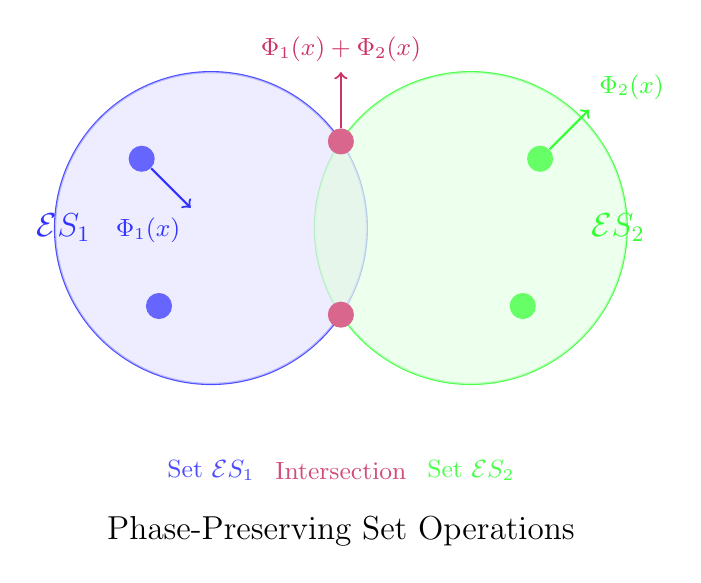
\begin{tikzpicture}[scale=1.1]
    % Define two circles with clear separation
    \def\radius{1.8}
    \coordinate (A) at (-1.5,0);
    \coordinate (B) at (1.5,0);
    
    % Fill intersection area
    \begin{scope}
        \clip (A) circle (\radius);
        \fill[purple!15] (B) circle (\radius);
    \end{scope}
    
    % Draw the two sets with clear boundaries
    \draw[blue!70, thick] (A) circle (\radius);
    \draw[green!70, thick] (B) circle (\radius);
    
    % Fill set areas (excluding intersection)
    \fill[blue!10, opacity=0.7] (A) circle (\radius);
    \fill[green!10, opacity=0.7] (B) circle (\radius);
    
    % Set labels positioned clearly outside circles
    \node[blue!80, font=\large] at (-3.2,0) {$\mathcal{E}\mathbb{S}_1$};
    \node[green!80, font=\large] at (3.2,0) {$\mathcal{E}\mathbb{S}_2$};
    
    % Elements in first set only (non-overlapping positions)
    \node[circle, fill=blue!60, minimum size=0.25cm] (e1) at (-2.3,0.8) {};
    \node[circle, fill=blue!60, minimum size=0.25cm] (e2) at (-2.1,-0.9) {};
    
    % Elements in second set only
    \node[circle, fill=green!60, minimum size=0.25cm] (e3) at (2.3,0.8) {};
    \node[circle, fill=green!60, minimum size=0.25cm] (e4) at (2.1,-0.9) {};
    
    % Elements in intersection (clearly separated)
    \node[circle, fill=purple!60, minimum size=0.25cm] (e5) at (0,1.0) {};
    \node[circle, fill=purple!60, minimum size=0.25cm] (e6) at (0,-1.0) {};
    
    % Phase arrows with clear spacing and labels
    \draw[->, blue!80, thick] (e1) -- +(-45:0.8) node[below left, font=\small] {$\Phi_1(x)$};
    \draw[->, green!80, thick] (e3) -- +(45:0.8) node[above right, font=\small] {$\Phi_2(x)$};
    
    % Coherent phase in intersection with clear positioning
    \draw[->, purple!80, thick] (e5) -- +(90:0.8) node[above, font=\small] {$\Phi_1(x) + \Phi_2(x)$};
    
    % Operation labels
    \node[font=\small, blue!70] at (-1.5,-2.8) {Set $\mathcal{E}\mathbb{S}_1$};
    \node[font=\small, green!70] at (1.5,-2.8) {Set $\mathcal{E}\mathbb{S}_2$};
    \node[font=\small, purple!70] at (0,-2.8) {Intersection};
    
    % Title
    \node[font=\large] at (0,-3.5) {Phase-Preserving Set Operations};
\end{tikzpicture}
\caption{Visualization of phase-preserving set operations, showing how phase information is preserved and combined when performing union and intersection operations}
\label{fig:phase_set_ops}
\end{figure}

\subsection{Orbital Differential Operators}

Set-theoretic operations in Elder Theory must account for orbital relationships, leading to the definition of orbital differential operators.

\begin{definition}[Orbital Differential]
For an Elder Set $\mathcal{E}\mathbb{S}$ with orbital relation $\mathcal{O}$, the orbital differential $\nabla_{\mathcal{O}}$ is an operator that measures the rate of change of properties with respect to orbital position.
\end{definition}

This orbital differential enables the definition of more complex operators:

\begin{definition}[Orbital Divergence and Curl]
For a vector field $\mathbf{F}$ defined on an Elder Set:
\begin{align}
\text{div}_{\mathcal{O}}(\mathbf{F}) &= \nabla_{\mathcal{O}} \cdot \mathbf{F} \\
\text{curl}_{\mathcal{O}}(\mathbf{F}) &= \nabla_{\mathcal{O}} \times \mathbf{F}
\end{align}
\end{definition}

These operators quantify the flow of information and rotation of phase within the orbital structure of the Elder Heliosystem, providing a mathematical formalism for critical system behaviors.

\section{Transfinite Cardinal Properties of Elder Sets}

\subsection{Aleph States in Elder Hierarchies}

The hierarchical nature of the Elder Heliosystem exhibits properties analogous to transfinite cardinal numbers in set theory, with important extensions.

\begin{theorem}[Elder Aleph Hierarchy]
The Elder Heliosystem exhibits a hierarchical structure that corresponds to the transfinite cardinal numbers $\aleph_0, \aleph_1, \ldots$ with the following correspondence:
\begin{enumerate}
    \item Elder entity: Cardinal class $\aleph_2$
    \item Mentor entities: Cardinal class $\aleph_1$
    \item Erudite entities: Cardinal class $\aleph_0$
\end{enumerate}
\end{theorem}

This hierarchy has profound implications for the information processing capabilities of the system:

\begin{corollary}[Information Capacity]
An Elder entity can process information of cardinality $\aleph_2$, strictly greater than the information processable by any finite collection of Mentors (of cardinality $\aleph_1$) or Erudites (of cardinality $\aleph_0$).
\end{corollary}

This provides a theoretical foundation for the Elder's ability to discover universal principles that transcend any finite collection of domains or tasks.

\begin{figure}[h]
\centering
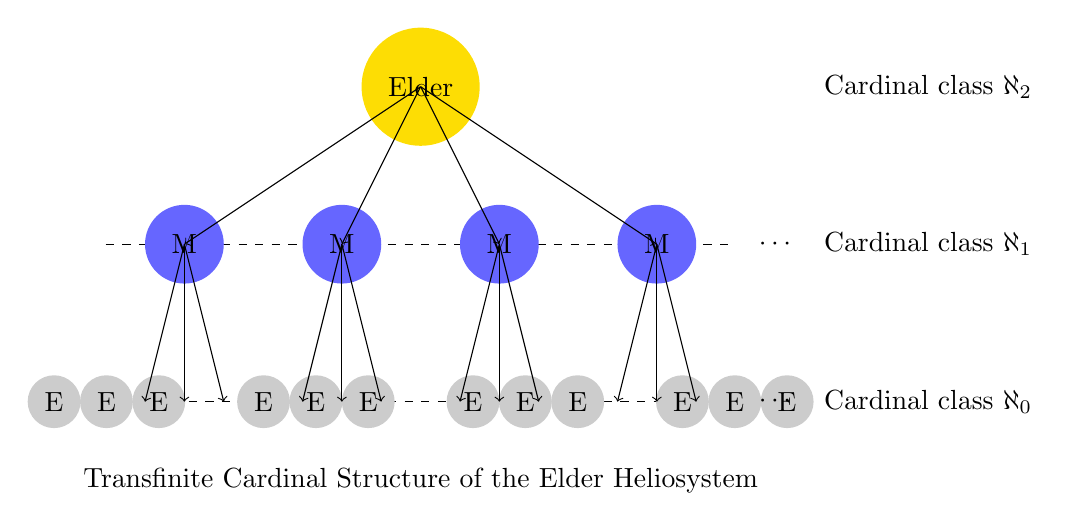
\begin{tikzpicture}[scale=1.0]
    % Set up cardinal levels
    \coordinate (elder) at (0,4);
    \coordinate (mentors) at (0,2);
    \coordinate (erudites) at (0,0);
    
    % Draw elder
    \node[circle, fill=yellow!80!orange, minimum size=1.5cm] at (elder) {Elder};
    \node[right] at (5,4) {Cardinal class $\aleph_2$};
    
    % Draw mentor level
    \draw[dashed] (-4,2) -- (4,2);
    \foreach \x in {-3,-1,1,3} {
        \node[circle, fill=blue!60, minimum size=1cm] at (\x,2) {M};
    }
    \node[right] at (5,2) {Cardinal class $\aleph_1$};
    \node at (4.5,2) {$\cdots$};
    
    % Draw erudite level
    \draw[dashed] (-4,0) -- (4,0);
    \foreach \x in {-4.655, -3.99, -3.325, -1.995, -1.33, -0.665, 0.665, 1.33, 1.995, 3.325, 3.99, 4.655} {
        \node[circle, fill=gray!40, minimum size=0.6cm] at (\x,0) {E};
    }
    \node[right] at (5,0) {Cardinal class $\aleph_0$};
    \node at (4.5,0) {$\cdots$};
    
    % Draw connections
    \foreach \x in {-3,-1,1,3} {
        \draw[->] (elder) -- (\x,2);
    }
    
    \foreach \x in {-3,-1,1,3} {
        \foreach \y in {\x-0.5,\x,\x+0.5} {
            \draw[->] (\x,2) -- (\y,0);
        }
    }
    
    % Title
    \node at (0,-1) {Transfinite Cardinal Structure of the Elder Heliosystem};
\end{tikzpicture}
\caption{The Elder Heliosystem hierarchy mapped to transfinite cardinal numbers, showing how each level of the hierarchy corresponds to a distinct aleph class}
\label{fig:aleph_hierarchy}
\end{figure}

\subsection{The Continuum Hypothesis in Phase Space}

The Elder Heliosystem offers a novel perspective on the Continuum Hypothesis, one of the most famous unresolved questions in classical set theory.

\begin{conjecture}[Phase Continuum Hypothesis]
In the Elder Heliosystem, there exists no set with cardinality strictly between that of the Erudites ($\aleph_0$) and the Mentors ($\aleph_1$), nor between the Mentors ($\aleph_1$) and the Elder ($\aleph_2$).
\end{conjecture}

This conjecture has important implications for the architecture of the system:

\begin{proposition}[Elder Architectural Optimality]
Assuming the Phase Continuum Hypothesis holds, the three-tier architecture of the Elder Heliosystem (Elder-Mentor-Erudite) represents the minimal hierarchical structure capable of spanning the full spectrum of knowledge representation.
\end{proposition}

\section{Orbital Zermelo-Fraenkel Axioms}

\subsection{Extended ZF Axioms for Elder Sets}

The foundational axioms of set theory, the Zermelo-Fraenkel (ZF) axioms, require extension to accommodate the phase and orbital properties of Elder Sets.

\begin{definition}[Orbital Zermelo-Fraenkel Axioms]
The Orbital ZF (OZF) axioms extend classical ZF axioms with:
\begin{enumerate}
    \item \textbf{Axiom of Phase}: Every element $x$ in an Elder Set has a well-defined phase $\Phi(x) \in [0, 2\pi)$.
    \item \textbf{Axiom of Orbital Relation}: For any two elements $x, y$ in an Elder Set, there exists a well-defined orbital relation $\mathcal{O}(x, y)$.
    \item \textbf{Axiom of Phase Coherence}: There exists a coherence function $C$ such that for any collection of elements with phases, $C$ determines their collective phase behavior.
    \item \textbf{Axiom of Hierarchical Containment}: If $x$ is orbitally contained by $y$ (denoted $x \in_{\mathcal{O}} y$), then the phase of $x$ is influenced by the phase of $y$ according to a gravitational influence function.
\end{enumerate}
\end{definition}

These axioms provide a rigorous set-theoretic foundation for Elder Theory that accounts for its unique phase and orbital properties.

\subsection{The Elder Choice Axiom}

The Axiom of Choice in classical set theory has an important analog in Elder Theory.

\begin{axiom}[Elder Choice Axiom]
Given any collection of non-empty Elder Sets, it is possible to select exactly one element from each set in a phase-coherent manner, meaning the selected elements collectively maximize phase coherence.
\end{axiom}

This axiom has profound implications for optimization processes in the Elder Heliosystem:

\begin{theorem}[Coherent Selection Theorem]
Under the Elder Choice Axiom, there exists an optimal selection of parameters across all domains that maximizes system-wide phase coherence. This selection corresponds to the global minimum of the Elder Loss function.
\end{theorem}

\section{Topological Properties of Elder Phase Space}

\subsection{Orbital Manifolds and Fiber Bundles}

The Elder Heliosystem's phase space exhibits rich topological structures that can be formalized using concepts from algebraic topology.

\begin{definition}[Orbital Manifold]
An Orbital Manifold $\mathcal{M}_{\mathcal{O}}$ is a smooth manifold equipped with an orbital metric derived from the orbital relation $\mathcal{O}$.
\end{definition}

\begin{theorem}[Phase Fiber Bundle Structure]
The phase space of the Elder Heliosystem forms a fiber bundle $\mathcal{E}$ with:
\begin{itemize}
    \item Base space $B$: The parameter space of entity positions
    \item Fiber $F$: The circle group $S^1$ representing phases
    \item Projection $\pi: \mathcal{E} \to B$ mapping each entity to its parameter configuration
\end{itemize}
\end{theorem}

This fiber bundle structure provides a formal framework for understanding how phase information is organized across the parameter space of the system.

\begin{figure}[h]
\centering
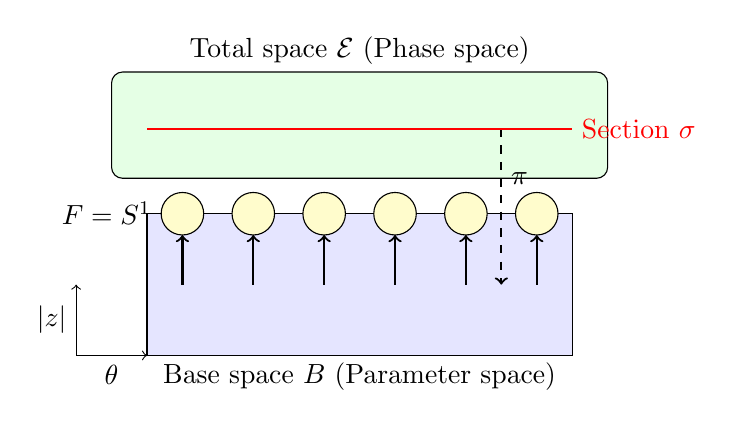
\begin{tikzpicture}[scale=0.9]
    % Base space
    \draw[fill=blue!10] (-3,-1) rectangle (3,1);
    \node at (0,-1.3) {Base space $B$ (Parameter space)};
    
    % Fibers
    \foreach \x in {-2.5,-1.5,-0.5,0.5,1.5,2.5} {
        \draw[fill=yellow!20] (\x,1) circle (0.3);
        \draw[->, thick] (\x,0) -- (\x,0.7);
    }
    
    % Total space (representation)
    \draw[fill=green!10, rounded corners] (-3.5,1.5) rectangle (3.5,3);
    \node at (0,3.3) {Total space $\mathcal{E}$ (Phase space)};
    
    % Projection
    \draw[->, thick, dashed] (2,2.2) -- (2,0);
    \node[right] at (2,1.5) {$\pi$};
    
    % Fiber label
    \node[left] at (-2.8,1) {$F = S^1$};
    
    % Section (a specific phase configuration)
    \draw[red, thick] (-3,2.2) -- (3,2.2);
    \node[red, right] at (3,2.2) {Section $\sigma$};
    
    % Coordinate systems
    \draw[->] (-4,-1) -- (-3,-1);
    \draw[->] (-4,-1) -- (-4,0);
    \node[below] at (-3.5,-1) {$\theta$};
    \node[left] at (-4,-0.5) {$|z|$};
\end{tikzpicture}
\caption{The Elder phase space as a fiber bundle, showing how phase information (fibers) is organized above the parameter space (base). A section $\sigma$ represents a specific phase configuration across all parameters.}
\label{fig:phase_fiber_bundle}
\end{figure}

\subsection{Cohomology of Phase Space}

The cohomological structure of the Elder phase space reveals important invariants that characterize its global properties.

\begin{definition}[Phase Cohomology]
The Phase Cohomology groups $H^n_{\Phi}(\mathcal{M}_{\mathcal{O}})$ of an Orbital Manifold are cohomology groups computed with respect to the phase-augmented differential $d_{\Phi} = d + i\Phi \wedge$.
\end{definition}

\begin{theorem}[Phase Cohomology Isomorphism]
The $n$-th Phase Cohomology group of the Elder Heliosystem is isomorphic to the direct sum:
\begin{equation}
H^n_{\Phi}(\mathcal{M}_{\mathcal{O}}) \cong H^n(B) \oplus H^{n-1}(B)
\end{equation}
where $H^n(B)$ is the standard $n$-th cohomology group of the base parameter space.
\end{theorem}

These cohomology groups characterize topological invariants of the Elder phase space, providing insights into its global structure and fundamental principles that govern the mathematical relationships within the Elder framework and constrain possible phase configurations.

\section{Category-Theoretic Formulation of Elder Theory}

\subsection{The Category of Elder Sets}

Category theory provides a natural language for expressing the relations and transformations in Elder Theory.

\begin{definition}[Category of Elder Sets]
The category $\mathbf{ElderSet}$ consists of:
\begin{itemize}
    \item Objects: Elder Sets $(\mathcal{E}\mathbb{S}, \Phi, \mathcal{O})$
    \item Morphisms: Phase-preserving and orbital-structure-preserving maps between Elder Sets
    \item Composition: Standard function composition
    \item Identity: Identity function on each Elder Set
\end{itemize}
\end{definition}

\subsection{Functorial Properties of Elder Hierarchies}

The hierarchical structure of the Elder Heliosystem can be formalized using functors between appropriate categories.

\begin{definition}[Elder Hierarchy Functor]
The Elder Hierarchy Functor $\mathcal{H}: \mathbf{ElderSet} \to \mathbf{ElderSet}$ maps an Elder Set to a higher-level Elder Set in the hierarchy, preserving structural relationships.
\end{definition}

\begin{theorem}[Adjoint Hierarchy Construction]
The Elder Hierarchy Functor $\mathcal{H}$ forms an adjoint pair with the Projection Functor $\mathcal{P}$:
\begin{equation}
\mathcal{H} \dashv \mathcal{P}
\end{equation}
This adjunction formally characterizes the relationship between higher and lower levels in the Elder hierarchy.
\end{theorem}

\subsection{Natural Transformations as Learning Processes}

Learning processes in the Elder Heliosystem can be formalized as natural transformations between functors.

\begin{definition}[Learning Natural Transformation]
A Learning Natural Transformation $\eta: F \Rightarrow G$ between functors $F, G: \mathbf{C} \to \mathbf{ElderSet}$ represents a coherent learning process that preserves structural relationships across all objects in the category $\mathbf{C}$.
\end{definition}

\begin{figure}[h]
\centering
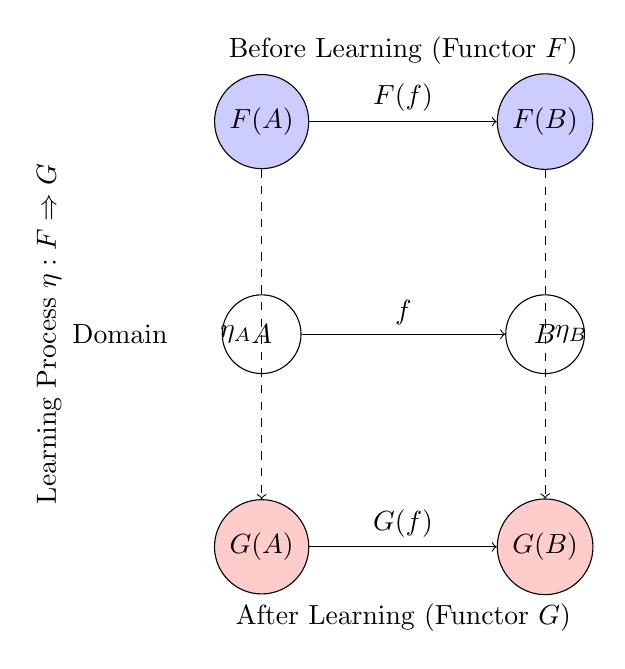
\begin{tikzpicture}[scale=0.9]
    % Two objects in source category
    \node[circle, draw, minimum size=1cm] (A) at (0,0) {$A$};
    \node[circle, draw, minimum size=1cm] (B) at (4,0) {$B$};
    \draw[->] (A) -- (B) node[midway, above] {$f$};
    
    % Images under functors
    \node[circle, draw, fill=blue!20, minimum size=1cm] (FA) at (0,3) {$F(A)$};
    \node[circle, draw, fill=blue!20, minimum size=1cm] (FB) at (4,3) {$F(B)$};
    \draw[->] (FA) -- (FB) node[midway, above] {$F(f)$};
    
    \node[circle, draw, fill=red!20, minimum size=1cm] (GA) at (0,-3) {$G(A)$};
    \node[circle, draw, fill=red!20, minimum size=1cm] (GB) at (4,-3) {$G(B)$};
    \draw[->] (GA) -- (GB) node[midway, above] {$G(f)$};
    
    % Natural transformation components
    \draw[->, dashed] (FA) -- (GA) node[midway, left] {$\eta_A$};
    \draw[->, dashed] (FB) -- (GB) node[midway, right] {$\eta_B$};
    
    % Labels
    \node at (2,4) {Before Learning (Functor $F$)};
    \node at (2,-4) {After Learning (Functor $G$)};
    \node at (-2,0) {Domain};
    \node[rotate=90] at (-3,0) {Learning Process $\eta: F \Rightarrow G$};
\end{tikzpicture}
\caption{Learning in the Elder Heliosystem formalized as a natural transformation between functors, showing how the learning process coherently transforms representations across all objects in the domain}
\label{fig:learning_natural_transform}
\end{figure}

This category-theoretic formulation provides a powerful framework for understanding the structural properties of learning processes in the Elder Heliosystem.

\section{Quantum Set Theory and Elder Phase Superposition}

\subsection{Quantum Superposition of Elder Sets}

The phase-based nature of Elder Sets has natural connections to quantum mechanics, leading to a quantum set-theoretic formulation.

\begin{definition}[Quantum Elder Set]
A Quantum Elder Set $\mathcal{Q}\mathcal{E}\mathbb{S}$ is an Elder Set where elements can exist in superpositions of phase states, represented as:
\begin{equation}
|\mathcal{Q}\mathcal{E}\mathbb{S}\rangle = \sum_i \alpha_i |x_i, \Phi_i\rangle
\end{equation}
where $\alpha_i$ are complex amplitude parameters that encode both magnitude and phase information for each computational path. These complex amplitude parameters satisfy the normalization constraint $\sum_i |\alpha_i|^2 = 1$ and determine the probability distribution over possible computation outcomes through their squared magnitudes $|\alpha_i|^2$.
\end{definition}

This quantum formulation enables the expression of phase uncertainty and entanglement between elements:

\begin{theorem}[Phase Entanglement]
In a Quantum Elder Set, elements can exhibit phase entanglement such that the phase of one element is correlated with the phase of another, even without direct orbital interaction.
\end{theorem}

\subsection{Measurement-Induced Phase Collapse}

The process of parameter activation in the Elder Heliosystem can be formalized using the concept of measurement-induced collapse from quantum mechanics.

\begin{definition}[Phase Collapse]
When a computation path is selected in the Elder Heliosystem, the superposition of potential phase states collapses to a specific configuration according to the probability distribution determined by the squared magnitudes of the complex amplitudes.
\end{definition}

This provides a theoretical foundation for the sparsity-inducing properties of the Elder Heliosystem, where only a small fraction of parameters are activated for any given computation.

\begin{corollary}[Sparse Activation]
The phase collapse process naturally induces sparsity in parameter activation, with the activation probability of each parameter determined by its phase alignment with the global system phase.
\end{corollary}

\section{Practical Implications for Elder Heliosystem Implementation}

\subsection{Set-Theoretic Optimization of Elder Architectures}

The set-theoretic properties of Elder Theory have direct implications for practical implementations of the Elder Heliosystem.

\begin{theorem}[Minimal Hierarchical Structure]
The minimal hierarchical structure required for a complete Elder Heliosystem is determined by the order type of transfinite cardinals needed to represent the desired information processing capacity.
\end{theorem}

This theorem guides the design of efficient Elder architectures by specifying the minimal hierarchical structure needed for a given application domain.

\subsection{Phase-Coherent Parameter Selection}

The Elder Choice Axiom provides guidance for parameter selection in practical implementations:

\begin{proposition}[Parameter Selection Strategy]
Optimal parameter selection in the Elder Heliosystem should maximize phase coherence across all levels of the hierarchy, which can be achieved through a gradient descent process on the phase coherence measure.
\end{proposition}

\begin{algorithm}[h]
\caption{Phase-Coherent Parameter Selection}
\begin{algorithmic}[1]
\State Initialize parameters $\theta$ randomly
\State Define phase coherence measure $C(\theta)$
\While{not converged}
\State Compute gradient $\nabla_{\theta} C(\theta)$
\State Update parameters: $\theta \leftarrow \theta + \eta \nabla_{\theta} C(\theta)$
\EndWhile
\State \Return $\theta$
\end{algorithmic}
\end{algorithm}

\section{Conclusion: Set Theory as the Foundation of Elder Theory}

The set-theoretic foundations presented in this chapter provide a rigorous mathematical basis for Elder Theory. By extending classical set theory with phase and orbital concepts, we establish a formal framework that:

\begin{enumerate}
    \item Explains the hierarchical structure of the Elder Heliosystem in terms of transfinite cardinals
    \item Formalizes the orbital and phase relationships that enable the system's unique properties
    \item Provides a topological characterization of the Elder phase space
    \item Enables category-theoretic formulations of learning processes
    \item Connects to quantum set theory through phase superposition principles
\end{enumerate}

These set-theoretic foundations not only provide theoretical justification for the Elder Heliosystem's architecture but also guide practical implementations by specifying optimal structures and algorithms based on rigorous mathematical principles.

\begin{theorem}[Foundational Adequacy]
The Orbital Zermelo-Fraenkel axiom system, augmented with the Elder Choice Axiom, provides a complete and consistent foundation for Elder Theory, sufficient to derive all essential properties of the Elder Heliosystem.
\end{theorem}

Future research will continue to explore the rich connections between set theory and Elder Theory, particularly in areas such as large cardinal axioms and their relationship to the information processing capabilities of higher-level Elder entities.